%\def\DEBUG{1}
\ifdefined\DEBUG
\documentclass[11pt,twoside]{mitthesis}
\usepackage{tikz}
\usepackage{circuitikz}
\usepackage{amsmath}
\usepackage{float}
\newcommand{\ohm}{$\Omega$ }
\begin{document}
\fi


\chapter{Hardware}
In this chapter, hardware system design is covered.
The hardware system is decomposed into its subsystems, and the design choices, specifications, and operation of those subsystems are explained.
The hardware system is composed of a set of eight breadboard rails connected to a node voltage reading system, a test voltage source system, a grounding system, and a 32-bit microcontroller development board.
The node voltage reading system is composed of a voltage multiplexer and an external A/D converter.
The test voltage source system is composed of an internal D/A converter, an external buffer, a current sensing amplifier, an external A/D converter, and eight high-side analog switches.
The grounding system is composed of eight N-channel MOSFETs, handled by the microcontroller.
A simplified block diagram is below:
\begin{figure}[h]
  \begin{center}
      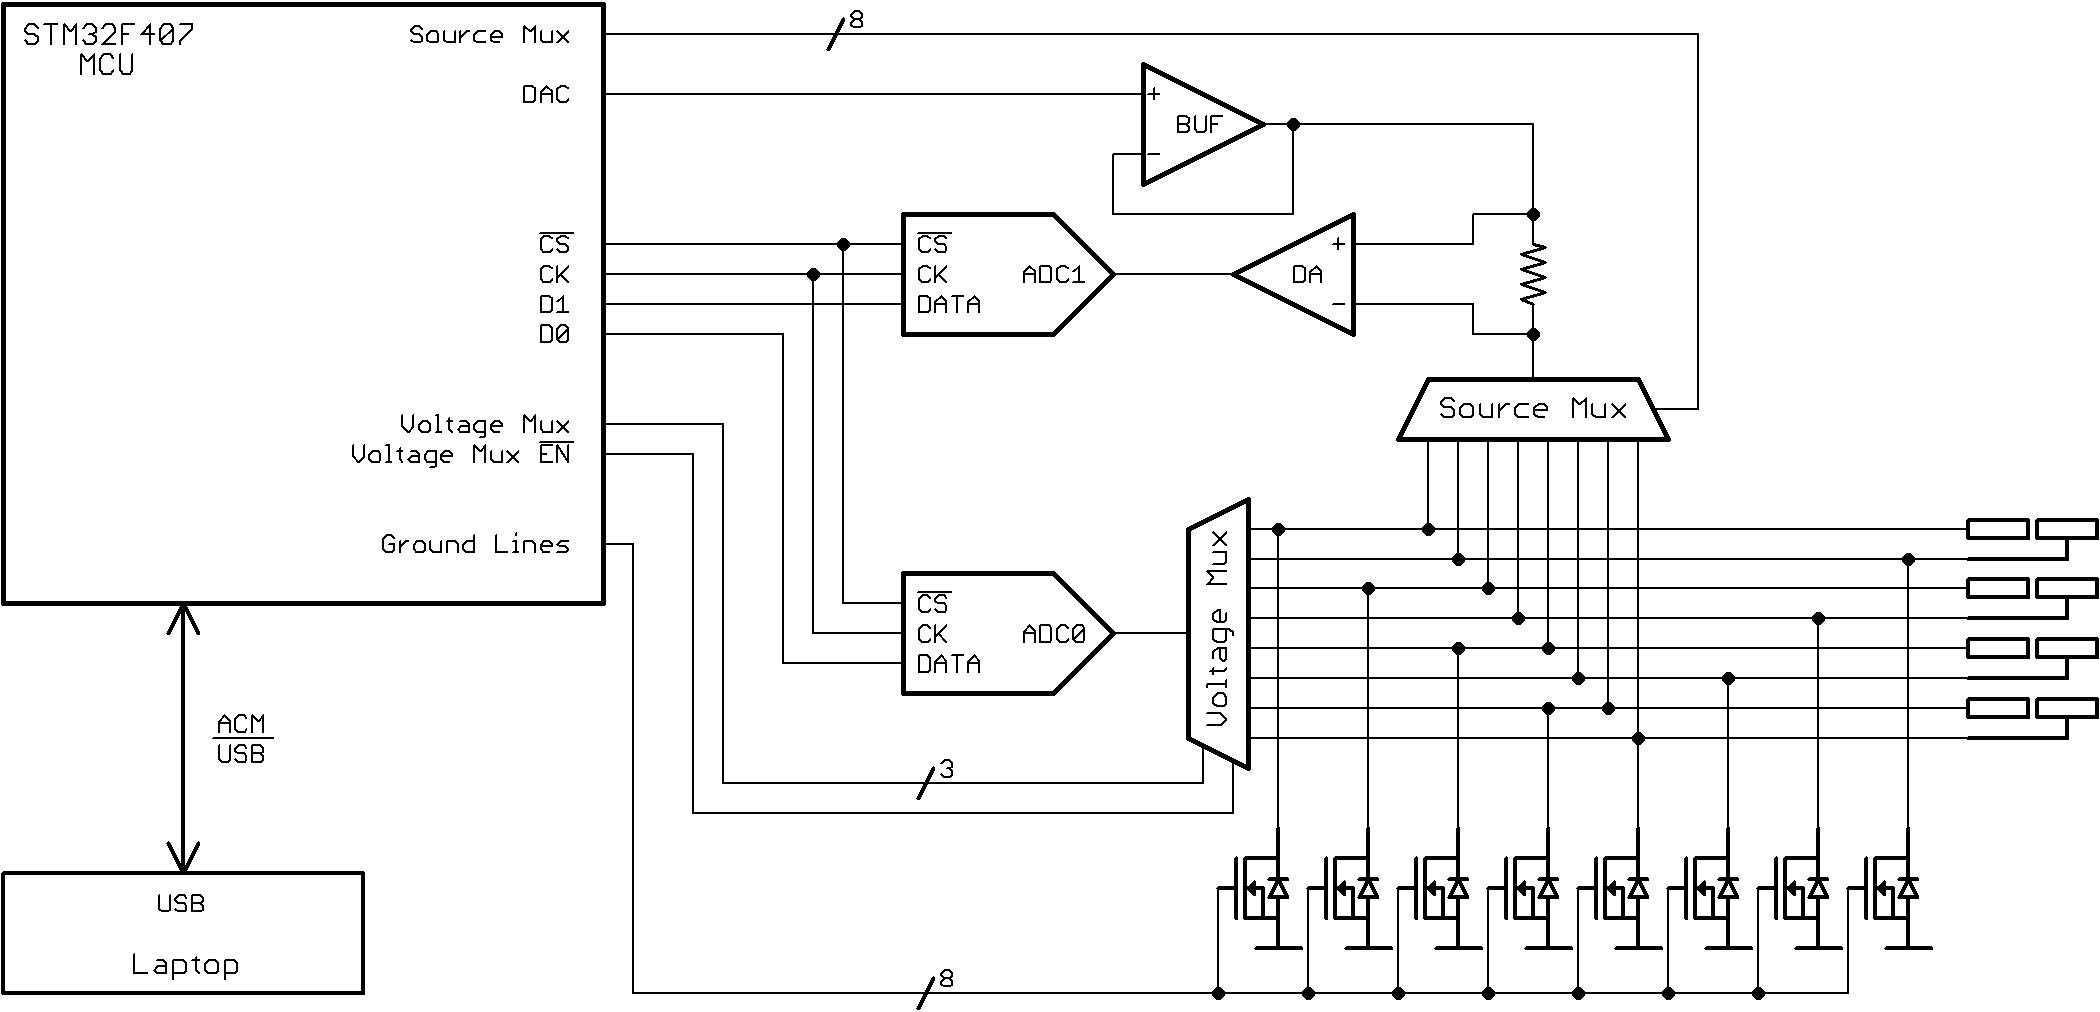
\includegraphics[width=.9\textwidth]{../circuit.png}
  \end{center}
  \caption{Simplified block diagram of hardware}
\end{figure}

\section{Node Voltage Reading}
An ADCS7476 12-bit A/D converter is used to measure the voltages at each node.
The ADCS7476 can sample up to 1MSPS with $\pm$1 LSB of total unadjusted error from $-40^o C$ to $85^o C$ and $<\pm 0.2$ LSB of error at $25^o C$.
No bits are wasted in the ADCS7476 A/D converter.
Additionally, the input circuitry to the ADC is a 100$\Omega$ resistor in series with a 26pF capacitor.  
This places a pole at 61MHz, causing a .03\% error at 100KHz and .3\% error at 1MHz.
The additional performance is well worth the additional cost of \$1.56375 in quantities of 1Ku.

\begin{figure}[h!]
  \begin{center}
      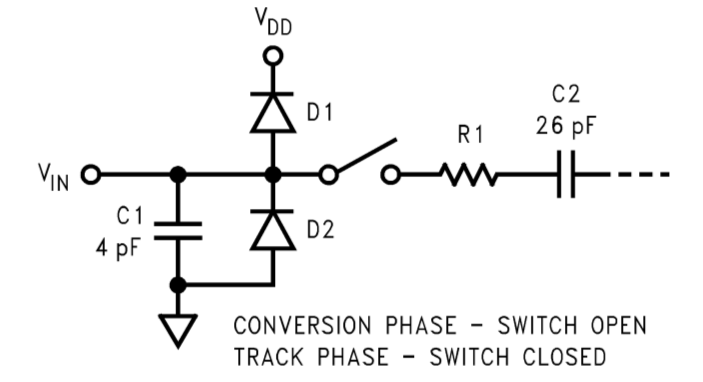
\includegraphics[width=.5\textwidth]{../adc-input-equiv.png}
      \caption{ADCS7476 Equivalent Input Circuit}
  \end{center}
\end{figure}


The ADC is connected to the common pin of a CD4051 1:8 analog multiplexer.
The multiplexer is connected to eight breadboard rails, which allows the ADC to measure the voltage on any of the eight rails, one rail at a time.

The CD4051 has about $200\Omega$ of series resistance and 30pF of output capacitance when its supply voltage is 12V, which places an additional pole at 26MHz, again well above the Nyquist frequency.

So far, the voltage-reading signal chain has two poles - one at 61MHz and one at 26MHz.

\subsection{Onboard A/D converters}
Although the STM32F407 has three onboard 12-bit A/D converters, their specifications are lacking.
Each is able to sample at 2MSPS, and it's possible to interleave them to attain a sampling rate of 6MSPS or higher if you're willing to throw away bits.
The total unadjusted error (offset error, gain error, differential linearity error, and integral linearity error) is between $\pm$2 LSB and $\pm$5 LSB.
With a minimum of $\pm$2 LSB's of error, the lowest significant two bits in the 12-bit A/D are virtually useless.
Another specification to consider is the input circuitry to the ADC.
The input circuitry to the ADC while it's in tracking mode looks like a 6K$\Omega$ resistor charging a 4pF capacitor.
This puts a pole at 6.6MHz, causing .3\% error in measurement at 100KHz, 3\% error in measurement at 1MHz, and 7\% at 3MHz.
When sampling at the maximum sample rate of 6MSPS, the ADC's input network begins to introduce significant error.
Granted, it's likely that there will be an alternative bandwidth bottleneck, this is still a metric of concern.
[DM00037051.pdf, pages 133-134]

\section{Signal Generator}

The STM32F407 has an onboard D/A converter that is good enough to use as a signal generator.
The onboard DAC is configured to output a cosine wavetable with a DC offset, as described in the next chapter.

\section{Test Voltage Current Sensing}

The DAC output is buffered by half of an MCP6L92 10MHz op-amp.
The onboard DAC can be configured with an optional onboard buffer, but the buffer limits the DAC output range from 0.2V to Vdd-0.2V.
Without the onboard buffer, the DAC output is 15k$\Omega$.
When configured as a voltage buffer, the MCP6L92 has an input impedance larger than 1G$\Omega$, resulting in no signal attenuation.

\begin{figure}[h!]
  \begin{center}
      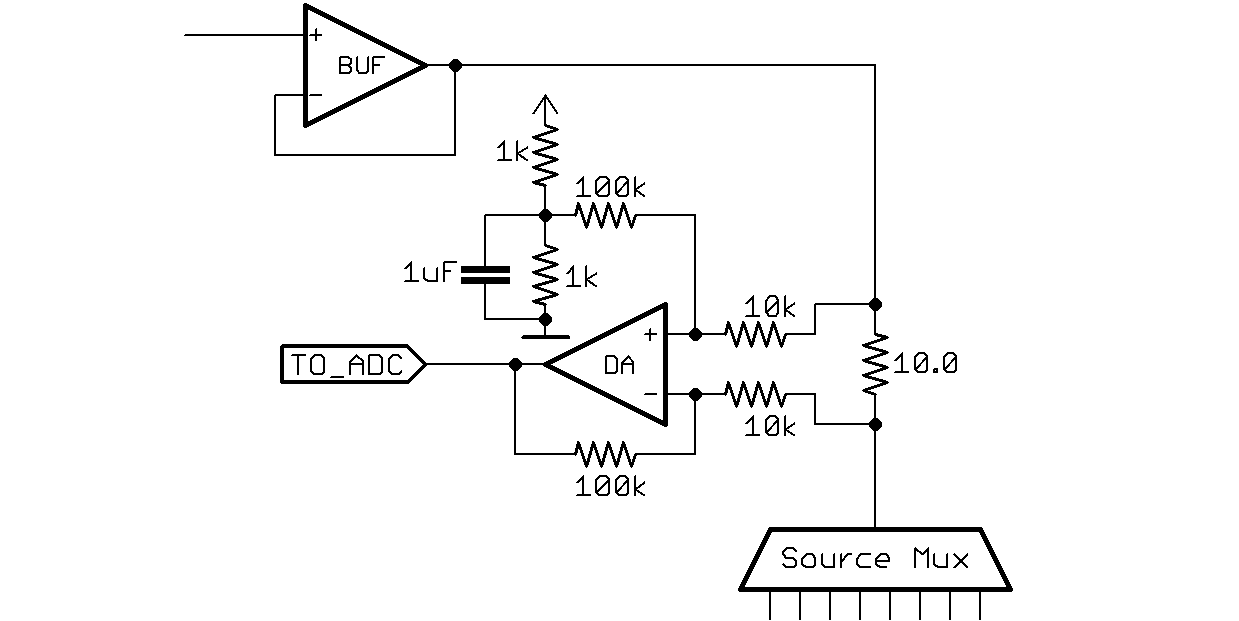
\includegraphics[width=.7\textwidth]{../DA.png}
      \caption{Difference Amplifier Schematic}
  \end{center}
\end{figure}

The buffer sources current through a 10.0\ohm, 1\% sense resistor, which can be switched onto any of the breadboard rails through an array of eight high-side switches.
The voltage across the sense resistor is measured by the other half of the MCP6L92 op-amp configured as a simple difference amplifier.
Using two 10k\ohm resistors and two 100k\ohm resistors, the difference amplifier is configured with a gain of 10.  

\begin{figure}[h!]
  \begin{center}
      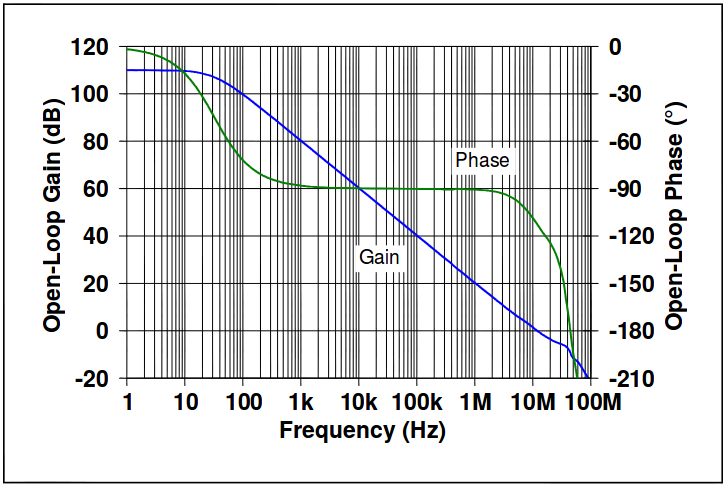
\includegraphics[width=.6\textwidth]{../opamp-bode.png}
      \caption{MCP6L92 Open Loop Bode Plot}
  \end{center}
\end{figure}

According to the MCP6L92 datasheet, the difference amplifier should have a -3dB bandwidth of 1MHz and plenty of phase margin driving the 100\ohm - 26pF input impedance to the current sense ADC.


\section{High-side Switches}

The high-side switches were selected for high-voltage operation, so that any rail of the breadboard could swing between 0 and 30V and there wouldn't be a problem.
The selected switches were Vishay DG468 normally open analog switches.
They have 9\ohm resistance and 76pF of capacitance in the on-state, 1nA of leakage current and 30pF of capacitance in the off-state.
The high and low side switches are the main limits of bandwidth due to their high amounts of input capacitance in both on and off states.


\section{Low-side Switches}

The low-side switches have a low logic-level threshold voltage, low drain-source on-resistance, can handle up to 30V, and are low-cost.
The IRLML2803 N-FETs have an $R_{DS_{ON}}$ of about 1\ohm with a $V_{GS}$ of 3.3V.
With 10V $V_{GS}$, $R_{DS_{ON}}$ drops to 250m\ohm.
The downside of these FETs is the high $C_{DS}$ that comes from a wide transistor.
$C_{DC}$ is on the order of 60pF for each transistor.
When combined with the additional capacitances mentioned above, each breadboard rail has a total of 140pF to ground.  
This has a significant impact on the maximum usable frequency for even moderate impedances on the breadboard.
For example, consider a 10k\ohm-10k\ohm resistor divider.
At 100kHz, the 140 pF capacitance on each rail has 11k\ohm of impedance.
\begin{figure}[h]
  \begin{center}
    \begin{circuitikz}[american]
    %\ctikzset{label/align = straight}
	
		\draw (0,0)
		node[sground] {}
		to[V,v^>=$V_t$] (0,3)
		to[short] (2,3)
		to[R,l_=$10k\Omega$] (2,1.5)
		to[R,l_=$10k\Omega$] (2,0)
		to[short] (0,0);
		\draw(2,1.5)
		to[short] (4,1.5)
		to[C,l_=$140pF$] (4,0)
		to[short] (2,0);
		\fill (2,1.5) circle (1mm);
		
		\draw (8,0)
		node[sground] {}
		to[sV,v^>=$V_tsin(100KHz)$] (8,3)
		to[short] (10,3)
		to[R,l_=$10k\Omega$] (10,1.5)
		to[R,l_=$10k\Omega$] (10,0)
		to[short] (8,0);
		\draw(10,1.5)
		to[short] (11,1.5)
		to[R,l=$11k\Omega$] (11,0)
		to[short] (10,0);
		\fill (10,1.5) circle (1mm);
		
    \end{circuitikz}
   \caption{Resistor Divider Parasitic Capacitance}
  \end{center}
\end{figure}

\section{PCB Mounted Breadboard}

Modern solderless breadboards are composed of three components: a plastic face, metal finger springs (rails), and a foam backing.
The finger springs are designed to fit snugly in the plastic face, which provides structure for the entire board.
The foam backing keeps the finger springs from being pushed out the back of the plastic face..

\begin{figure}[h!]
  \begin{center}
      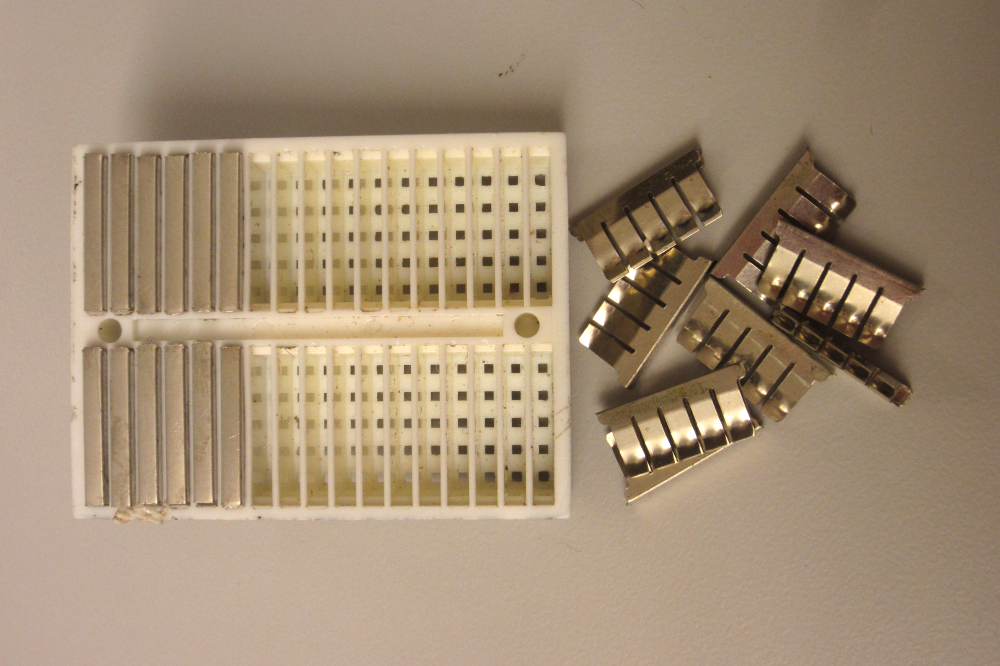
\includegraphics[width=.6\textwidth]{../bb-rails2.png}
      \caption{Solderless breadboard plastic face with finger spring rails removed}
  \end{center}
\end{figure}

A breadboard can be mounted to a PCB by removing the foam backing and surface mount soldering the finger springs to a PCB, then pressing the plastic face onto the mounted rails
Initial tests of this technique involved small numbers of finger springs hand-soldered one-by-one to a PCB, using nail polish as soldermask.

\begin{figure}[H]
  \begin{center}
      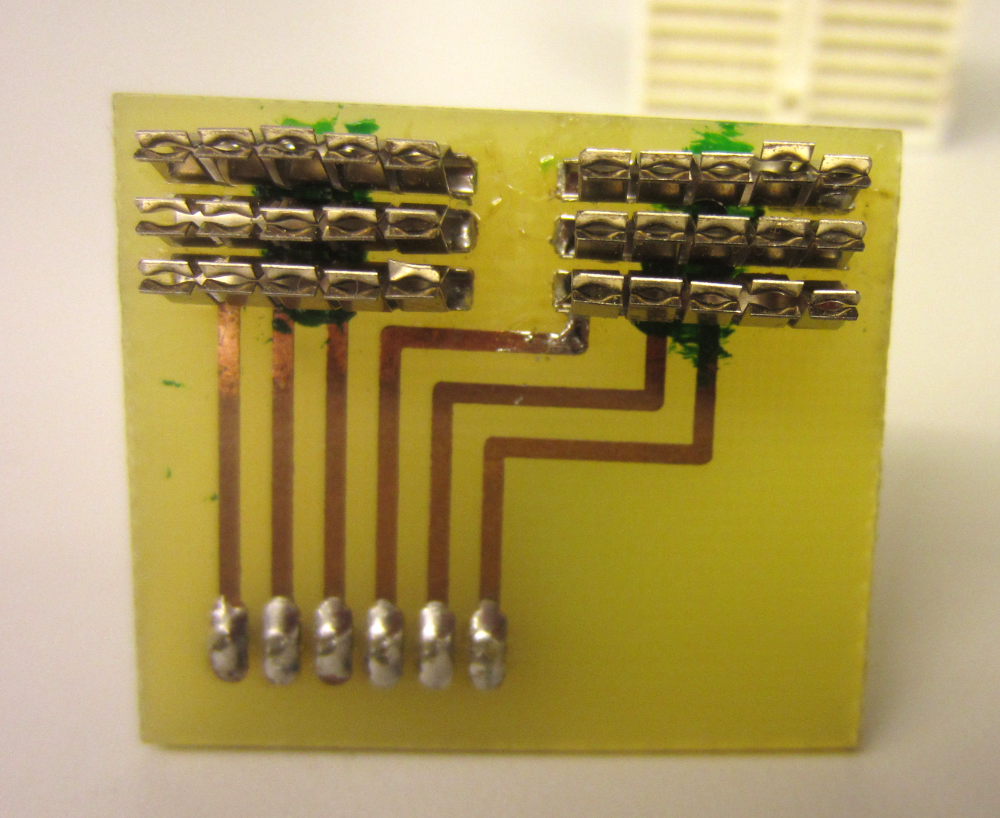
\includegraphics[width=.8\textwidth]{../bb-proto-1.png}
      \caption{Breadboard rails hand-mounted on copper clad PCB}
  \end{center}
\end{figure}

The results of these tests were promising, but alignment proved to be an issue.
To mitigate this, a finger spring jig was 3d-printed to loosely hold each finger spring in precise alignment for PCB mounting.
\begin{figure}[H]
  \begin{center}
      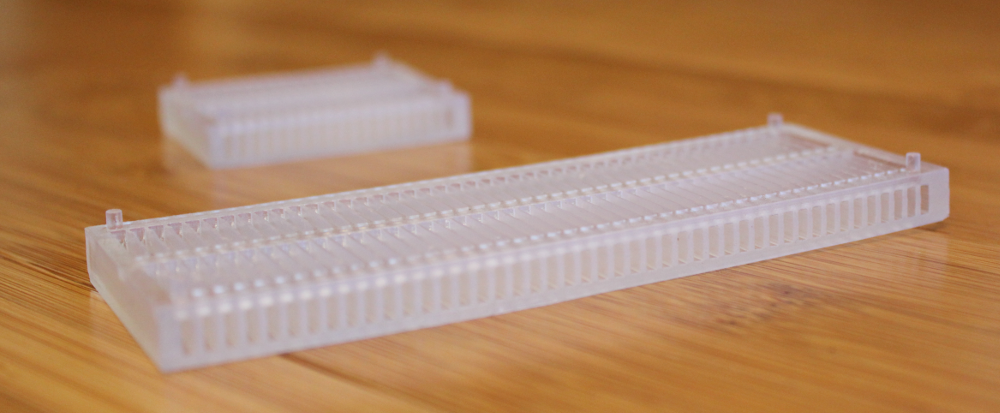
\includegraphics[width=.9\textwidth]{../bb-18-45.png}
      \caption{3D printed finger spring jigs}
  \end{center}
\end{figure}

\begin{figure}[H]
  \begin{center}
      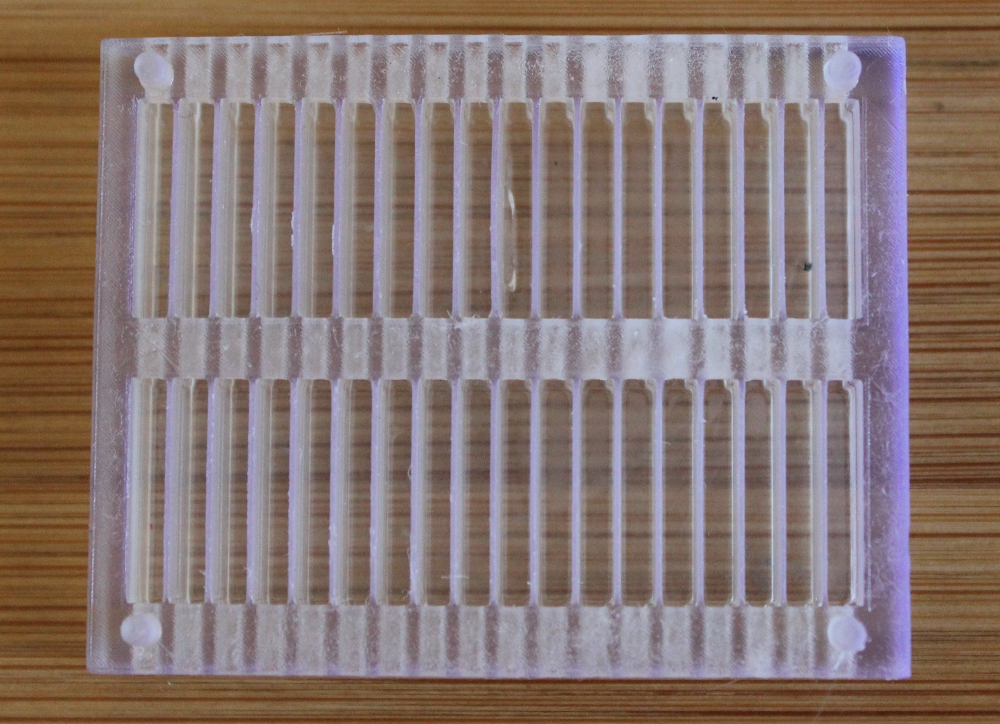
\includegraphics[width=.6\textwidth]{../bb-18.png}
      \caption{Top view of 36-position finger spring jig}
  \end{center}
\end{figure}

\begin{figure}[H]
  \begin{center}
      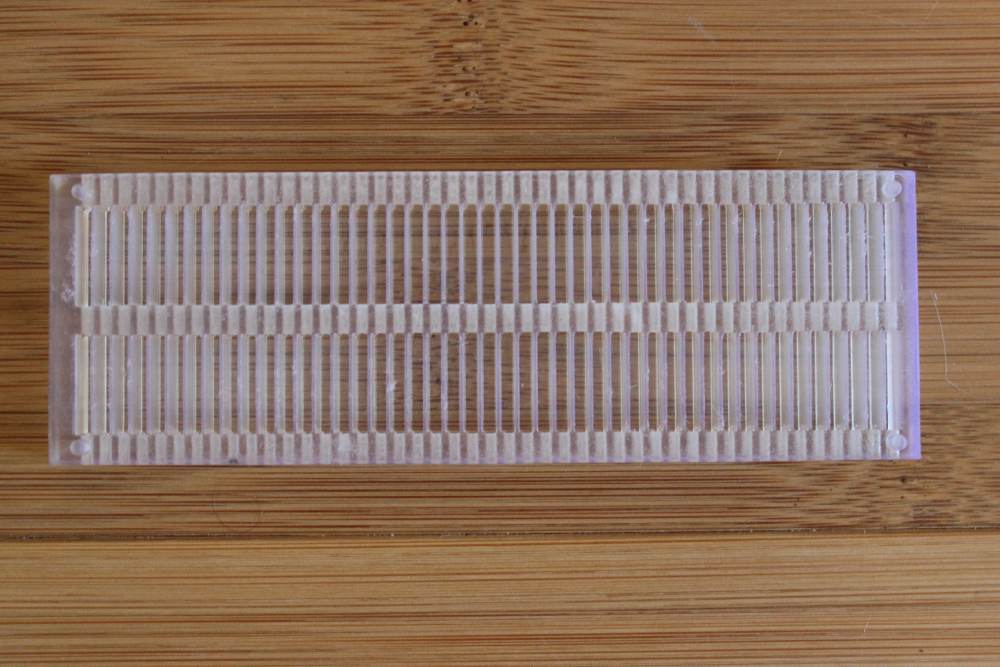
\includegraphics[width=.9\textwidth]{../bb-45.png}
      \caption{Top view of 90-position finger spring jig}
  \end{center}
\end{figure}

The finger spring jig was designed in openSCAD and has four alignment pegs to mate with alignment holes on a PCB.
To assemble a PCB mounted breadboard, the finger spring rails are removed from the breadboard and inserted into the finger spring jig.
\begin{figure}[H]
  \begin{center}
      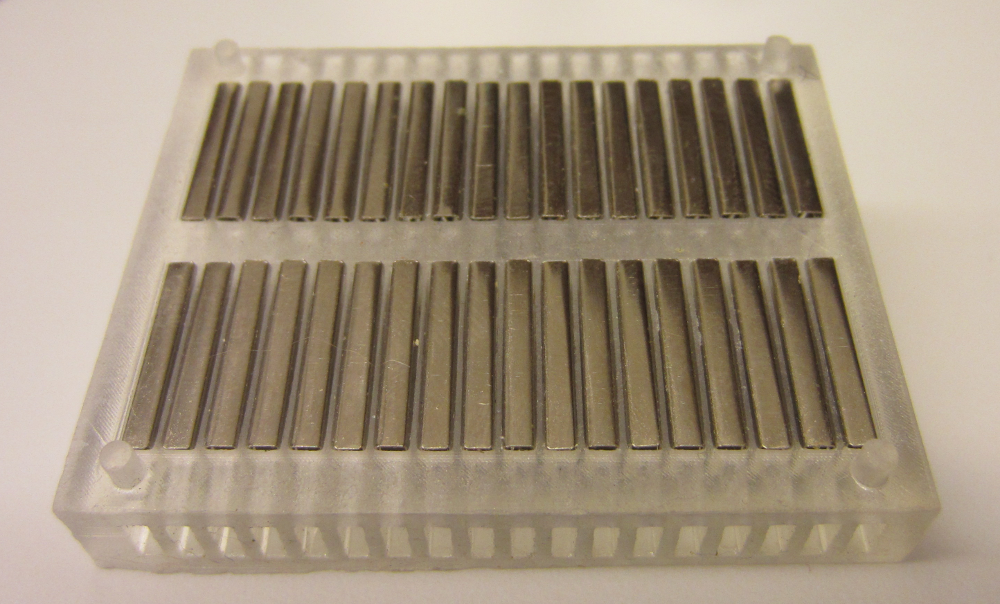
\includegraphics[width=.8\textwidth]{../bb-w-rails.png}
      \caption{Fully loaded 36-position finger spring jig}
  \end{center}
\end{figure}
Once all of the rails are placed, a dot of super glue is dispensed in the center of each finger spring, between two dots of solderpaste.
The rails are then adhered to the PCB by pressing the PCB upside-down onto the finger spring jig while the alignment pegs are properly mated with the alignment holes in the PCB.
This ensures that the array of finger spring rails are aligned with the pads on the PCB.
After about ten seconds the rails adhere to the PCB and the PCB can be carefully separated from the finger spring jig.
Finally the assembly is reflowed with hot air or in a reflow oven, and the plastic faceplate can be pressed on.
\begin{figure}[H]
  \begin{center}
      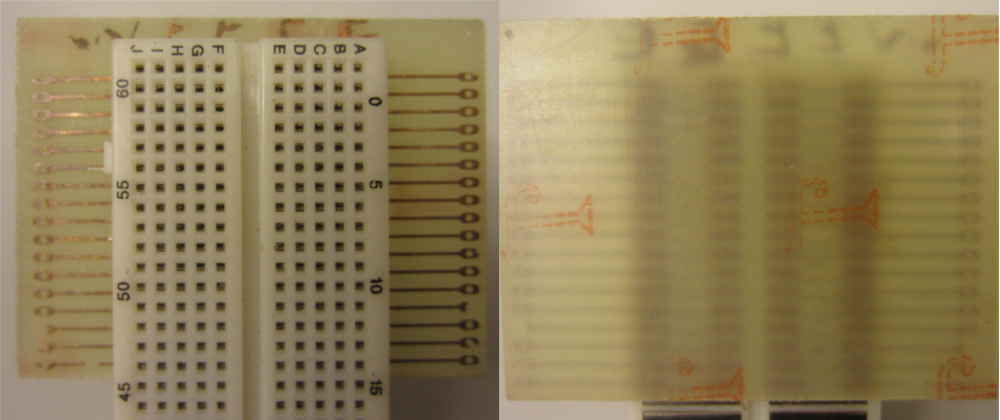
\includegraphics[width=.8\textwidth]{../bb-mount.png}
      \caption{Front and back of PCB mounted breadboard}
  \end{center}
\end{figure}

\section{Hardware Prototypes}

A number of prototype hardware subsystems were built to test various parts of the RLC network identifying breadboard.
All of these systems were designed and built by hand at the MIT Electronics Research Society [MITERS] facilities.

\begin{figure}[h]
  \begin{center}
      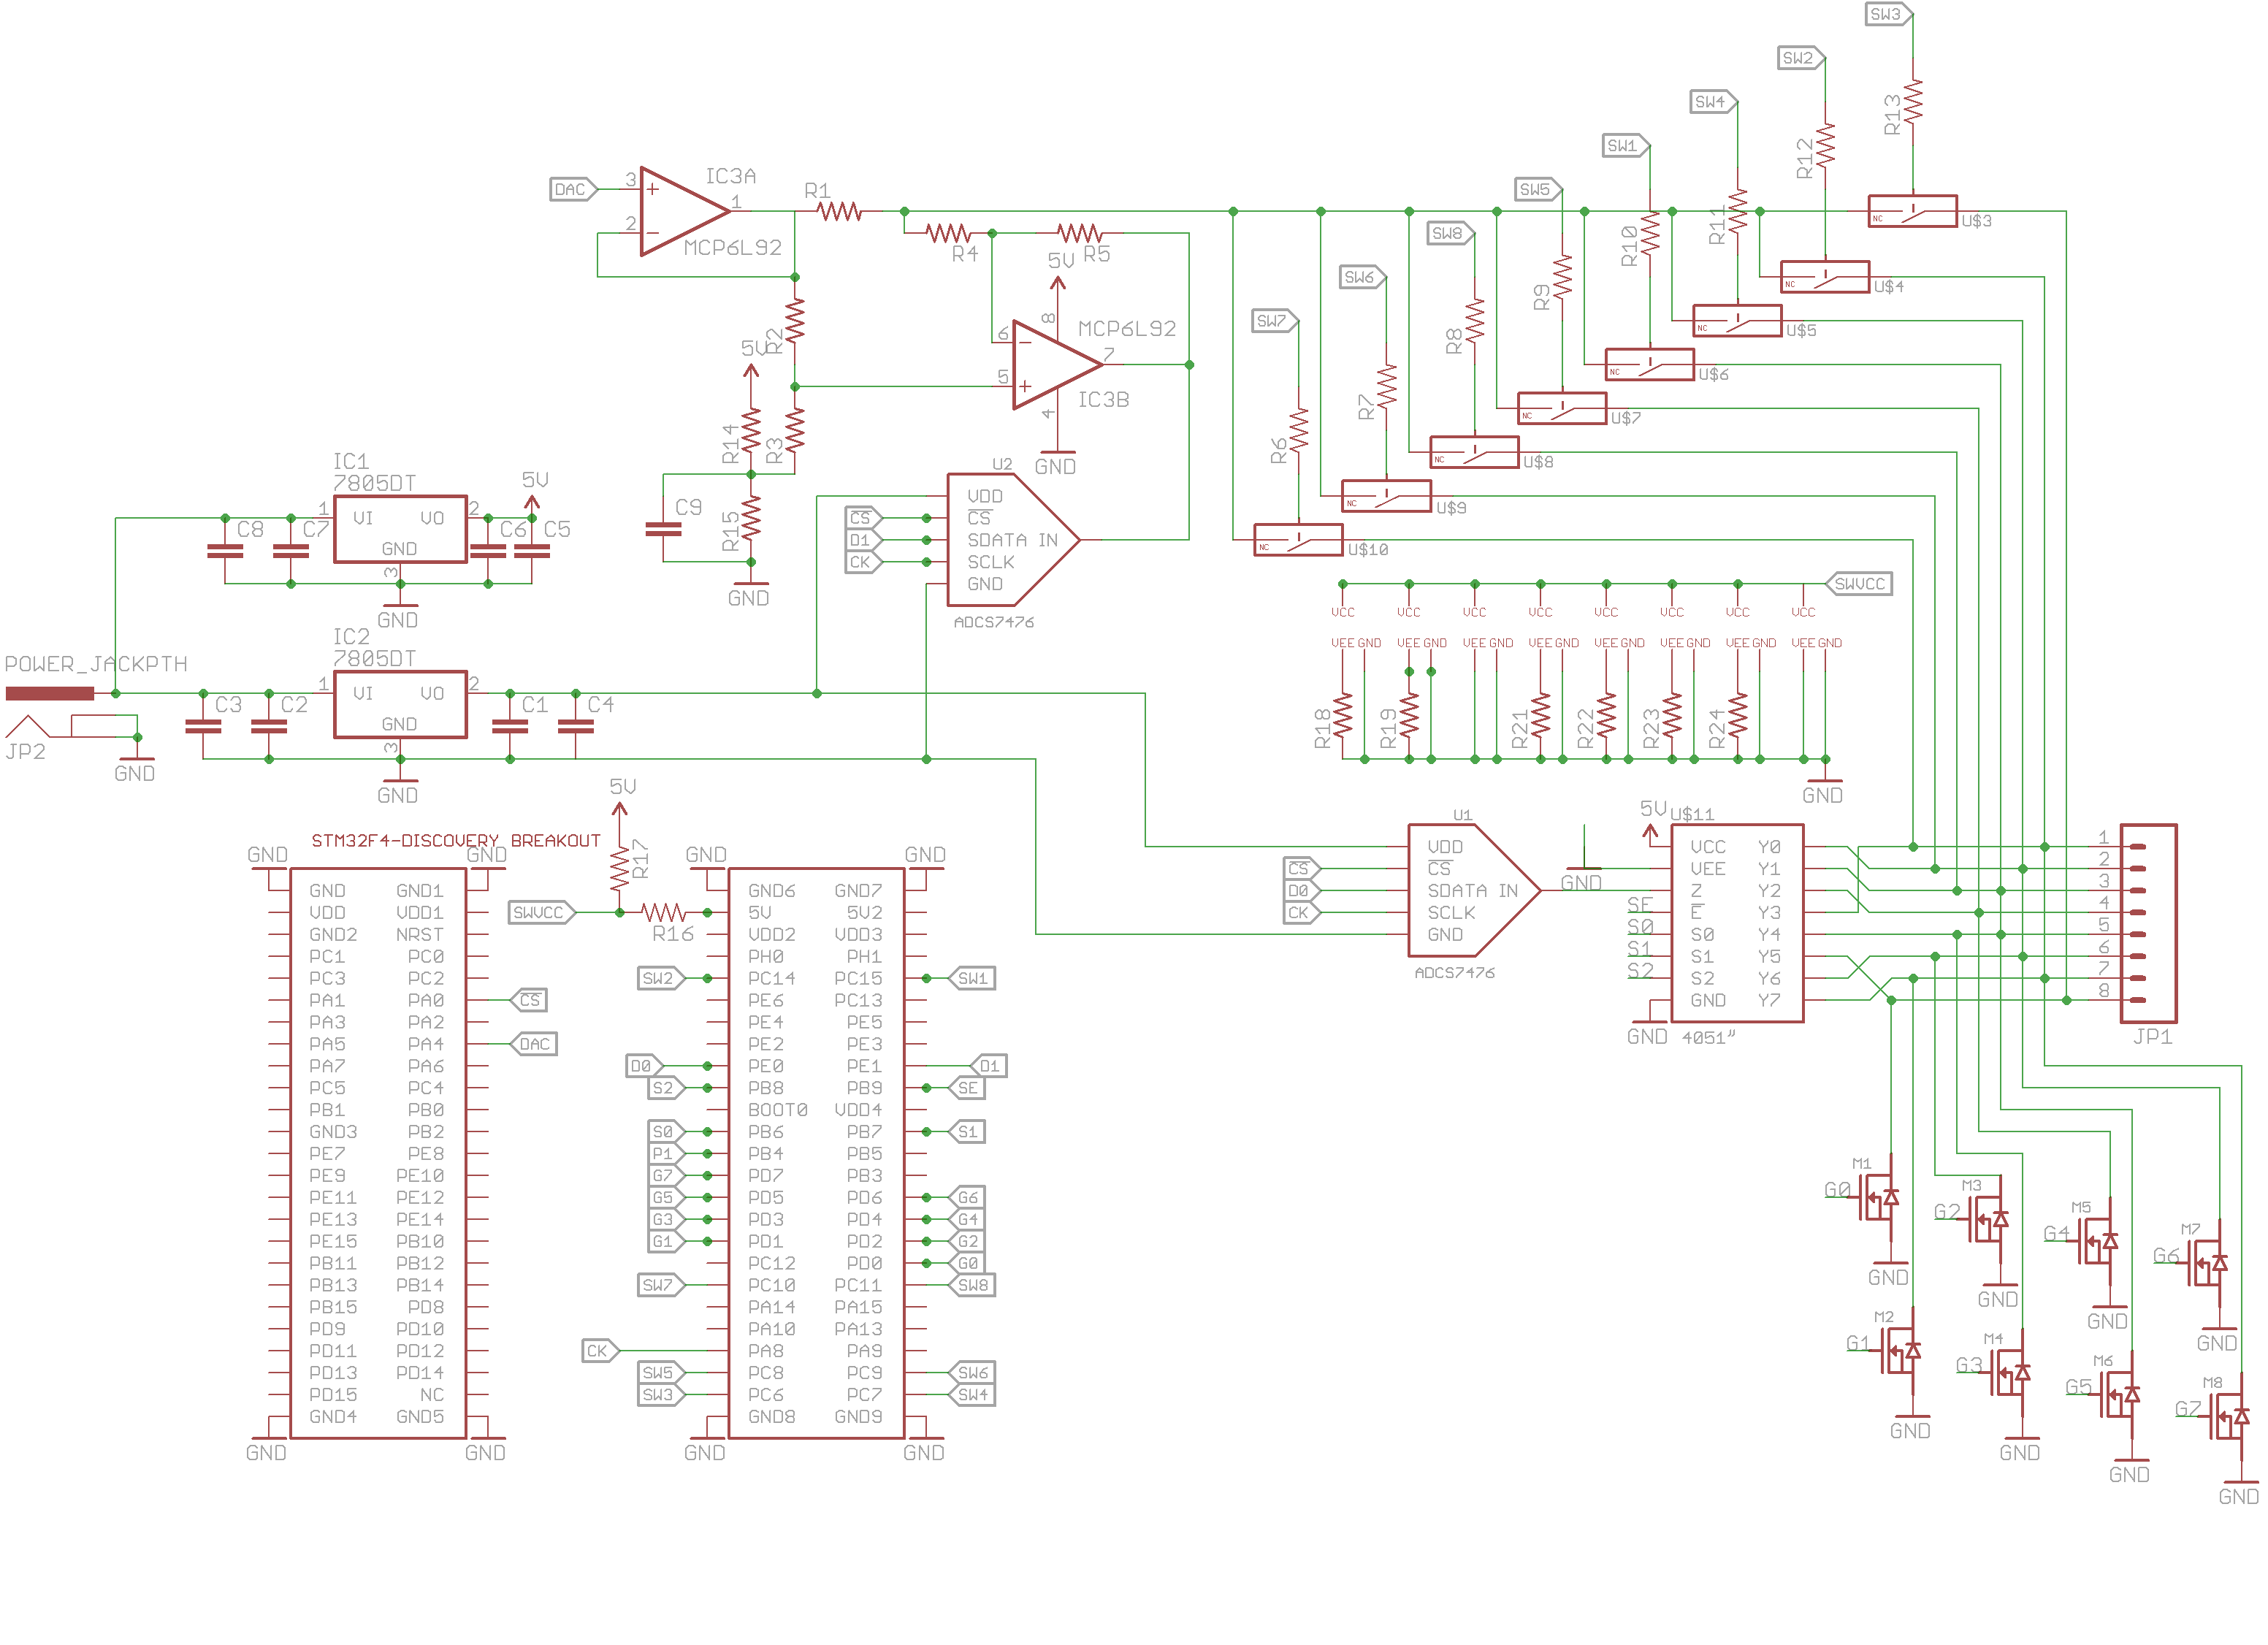
\includegraphics[width=1.08\textwidth, angle =90]{../schem1.png}
      \caption{Schematic of full hardware system}
  \end{center}
\end{figure}

\begin{figure}[h]
  \begin{center}
      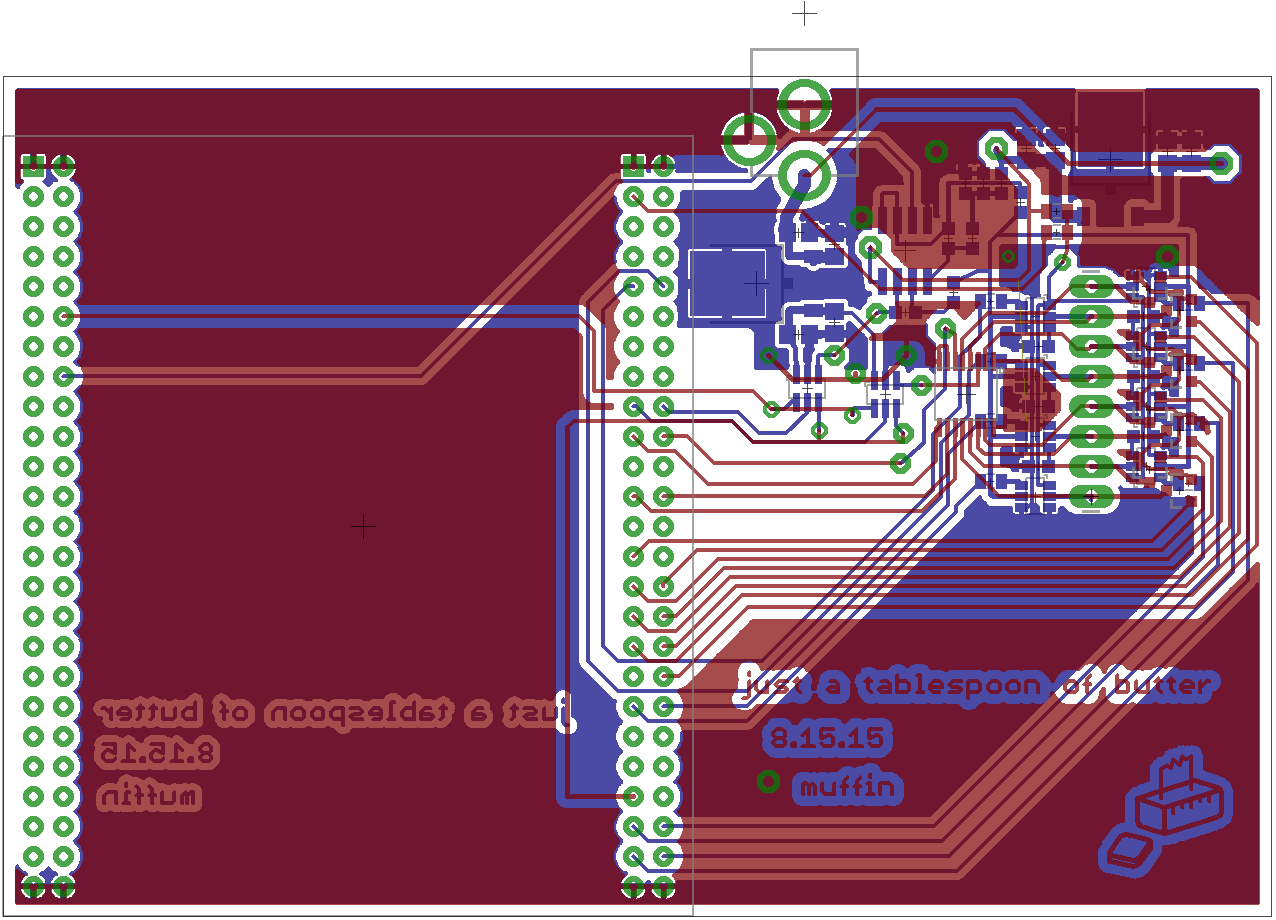
\includegraphics[width=.9\textwidth]{../layout-tb.png}
      \caption{Layout of full hardware system}
  \end{center}
\end{figure}

\begin{figure}[h]
  \begin{center}
      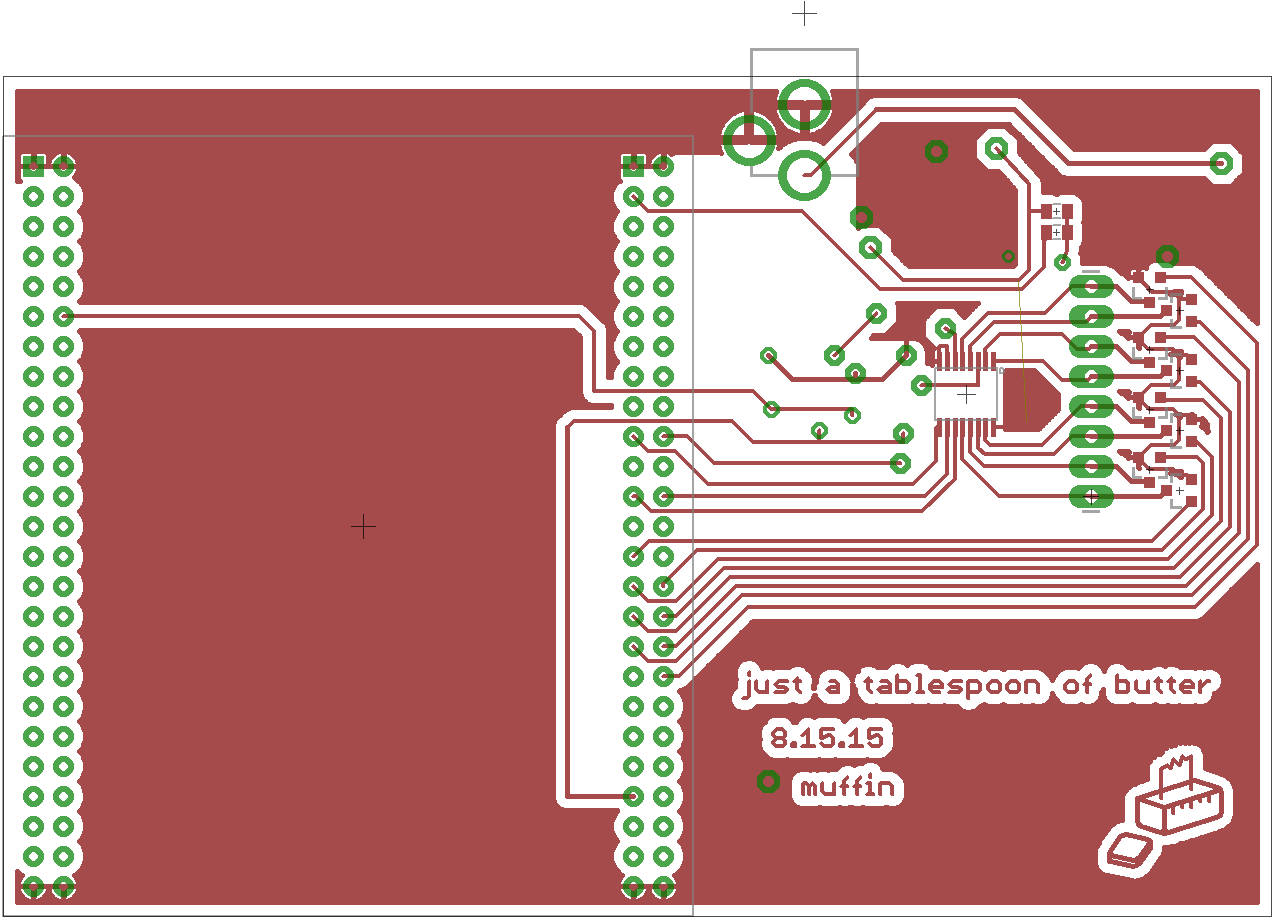
\includegraphics[width=.9\textwidth]{../layout-t.png}
      \caption{Top layer of full hardware system}
  \end{center}
\end{figure}

\begin{figure}[h]
  \begin{center}
      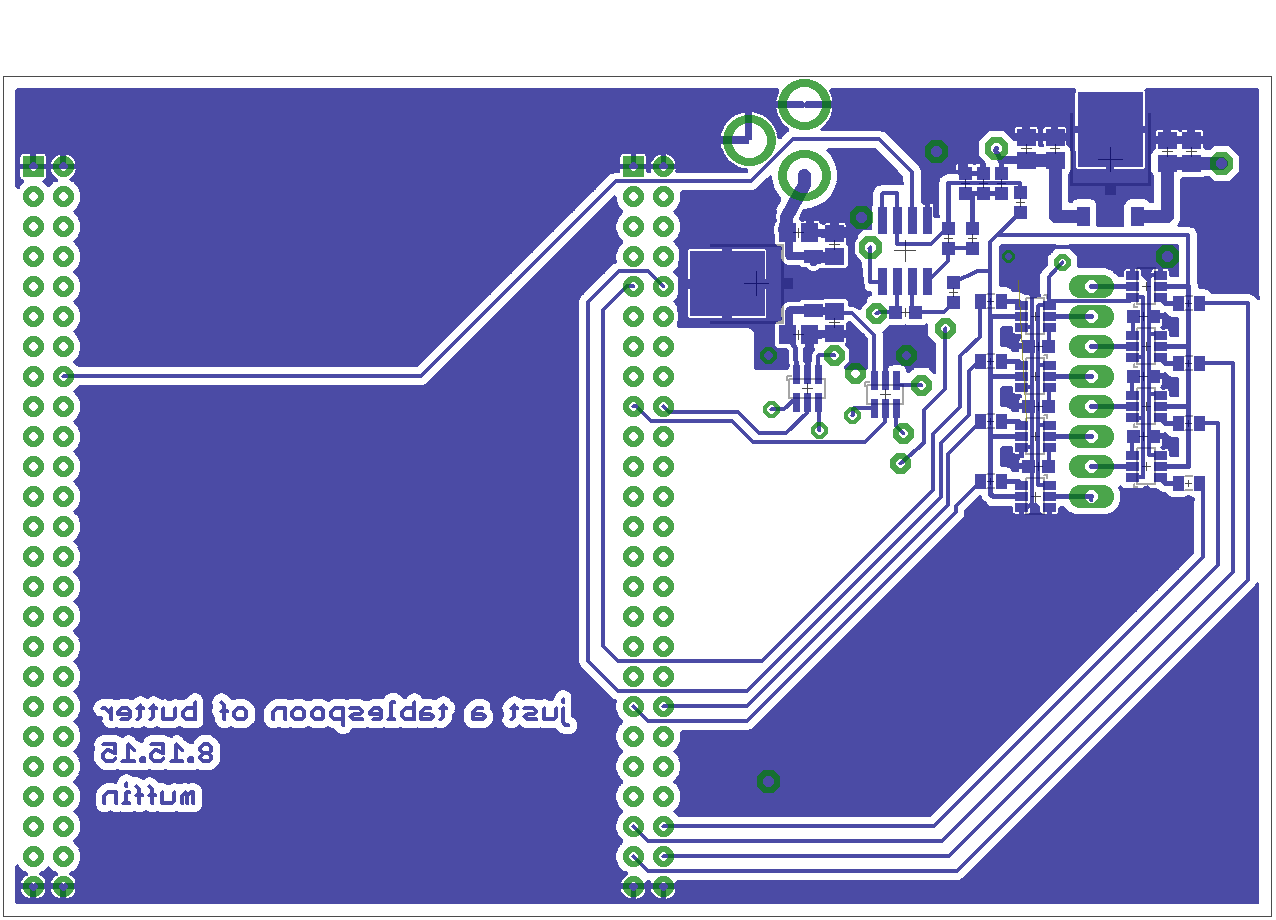
\includegraphics[width=.9\textwidth]{../layout-b.png}
      \caption{bottom layer of full hardware system}
  \end{center}
\end{figure}

\begin{figure}[h]
  \begin{center}
      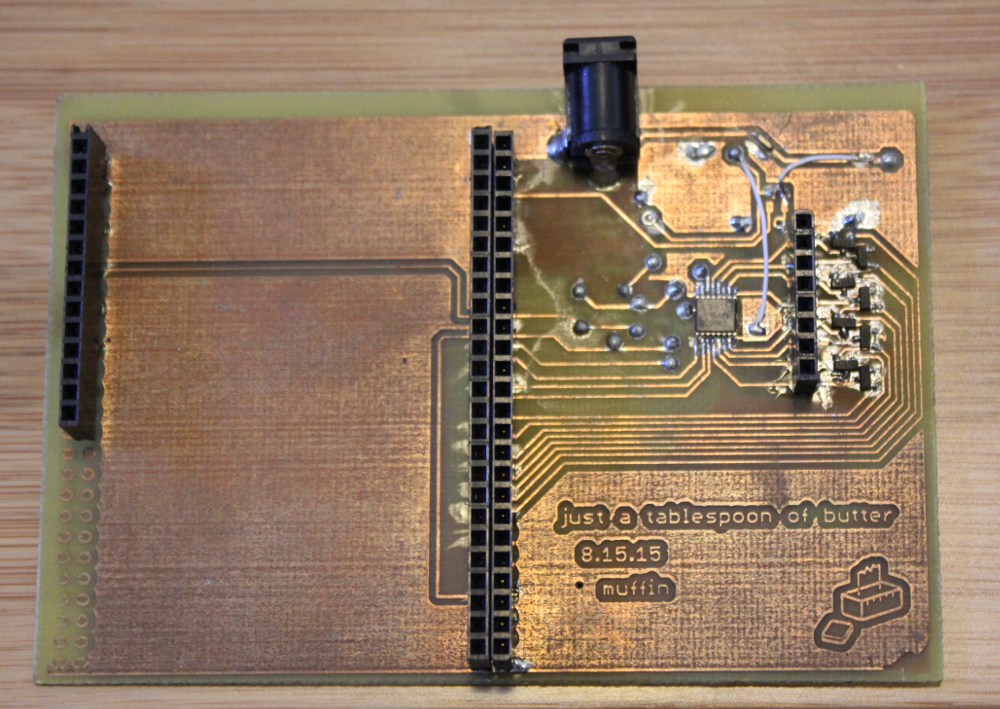
\includegraphics[width=.85\textwidth]{../butter-top.png}
      \caption{Top side of completed hardware system - power jack, voltage reading multiplexer, low-side switches, and 8-pin breadboard header are visible.}
  \end{center}
\end{figure}

\begin{figure}[h]
  \begin{center}
      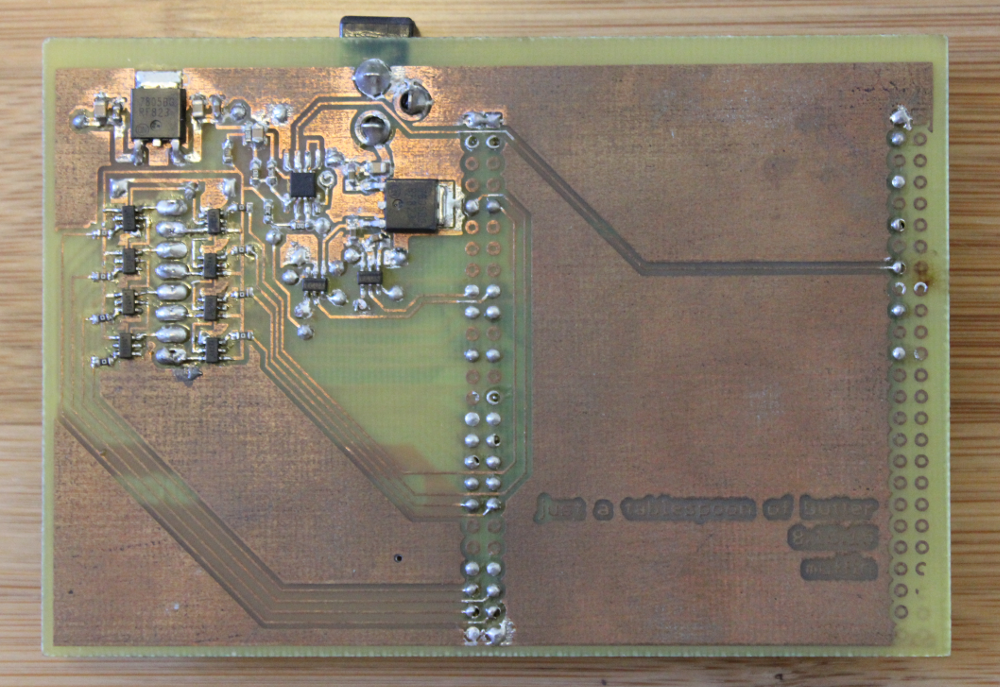
\includegraphics[width=.85\textwidth]{../butter-bot.png}
      \caption{Bottom side of completed hardware system - voltage regulators, A/D converters, high-side switches, and current-sense amplifier are visible}
  \end{center}
\end{figure}

\begin{figure}[h]
  \begin{center}
      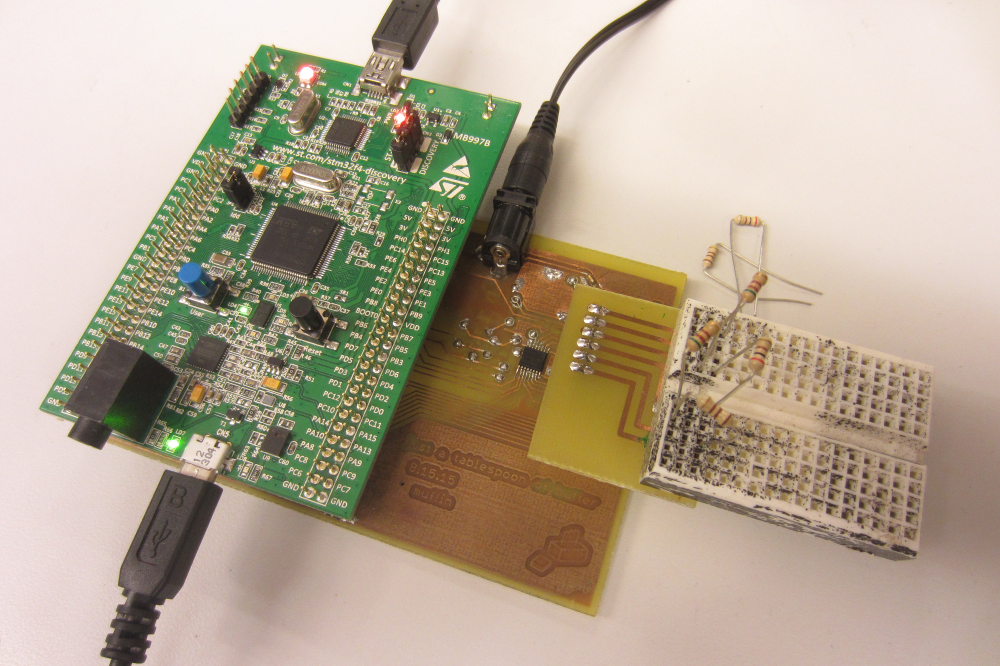
\includegraphics[width=\textwidth]{../system.png}
      \caption{8-node circuit sensing breadboard in operation}
  \end{center}
\end{figure}


\ifdefined\DEBUG
\end{document}
\fi
